\documentclass[11pt,letterpaper,twoside]{article}

\usepackage[utf8]{inputenc}
\usepackage[spanish,mexico]{babel}
\usepackage[T1]{fontenc}
\usepackage{listings}
\usepackage{hyperref}
\hypersetup{colorlinks=false}
\usepackage{lscape}
\usepackage{subfigure}
\usepackage{amsmath}
\usepackage{amssymb}
\usepackage{graphicx}
\usepackage{epstopdf}
\usepackage{float}
\usepackage[colorinlistoftodos]{todonotes}

% Paquetes adicionales para mejorar portada e introducción
\usepackage{xcolor}
\usepackage{tcolorbox}
\tcbuselibrary{skins,breakable,theorems}
\usepackage{tikz}
\usepackage{booktabs}
\usepackage{enumitem}
\usepackage{colortbl}
\usepackage{array}

% Ruta de las figuras generadas por el script de Python
\graphicspath{{img/}}

% Definición de colores institucionales
\definecolor{azulutez}{RGB}{0,51,102}
\definecolor{grisinstitucional}{RGB}{89,89,89}
\definecolor{fondoclaro}{RGB}{245,247,250}
\definecolor{verderesultado}{RGB}{0,102,51}
\definecolor{naranjaejercicio}{RGB}{204,102,0}

% Definición de entornos tcolorbox

% Entorno: Definición
\newtcolorbox[auto counter,number within=section]{definicion}[1][]{
    enhanced,
    colback=fondoclaro,
    colframe=azulutez,
    coltitle=white,
    fonttitle=\bfseries,
    title=Definición~\thetcbcounter\ifstrempty{#1}{}{: #1},
    boxrule=1pt,
    arc=2mm,
    left=8pt,
    right=8pt,
    top=6pt,
    bottom=6pt,
    breakable
}

% Entorno: Resultado (caja destacada para respuestas)
\newtcolorbox{resultado}{
    enhanced,
    colback=verderesultado!5,
    colframe=verderesultado,
    boxrule=1.5pt,
    arc=2mm,
    left=8pt,
    right=8pt,
    top=6pt,
    bottom=6pt
}

% Entorno: Nota
\newtcolorbox{nota}[1][]{
    enhanced,
    colback=fondoclaro,
    colframe=grisinstitucional!50,
    coltitle=grisinstitucional,
    fonttitle=\bfseries,
    title=\ifstrempty{#1}{Nota}{#1},
    boxrule=0.5pt,
    arc=2mm,
    left=8pt,
    right=8pt,
    top=6pt,
    bottom=6pt,
    breakable
}

% Entorno: Técnica
\newtcolorbox{tecnica}[1][]{
    enhanced,
    colback=azulutez!5,
    colframe=azulutez!70,
    coltitle=azulutez,
    fonttitle=\bfseries,
    title=\ifstrempty{#1}{Técnica}{#1},
    boxrule=0.5pt,
    arc=2mm,
    left=8pt,
    right=8pt,
    top=6pt,
    bottom=6pt,
    breakable
}

\usepackage{anysize}
\marginsize{2cm}{2cm}{1cm}{2cm}

\title{Actividad Integradora: Predicción del nivel de burnout estudiantil a partir del uso de IA generativa}

\author{Equipo 9C}

\renewcommand{\baselinestretch}{1.15}
\begin{document}
\parindent=0mm
\begin{titlepage}

\newcommand{\programa}{Ingeniería en Desarrollo y Gestión de Software}
\newcommand{\materia}{Extracción del conocimiento en Bases de datos}
\newcommand{\profesor}{VIRNA VIRIDIANA VELA RINCÓN}
\newcommand{\grupo}{9\textsuperscript{o} C}
\newcommand{\ciudad}{Emiliano Zapata, Morelos, México.}

% Fondo decorativo con TikZ
\begin{tikzpicture}[remember picture, overlay]
    % Franja superior
    \fill[azulutez] (current page.north west) rectangle ([yshift=-2.5cm]current page.north east);
    % Franja inferior
    \fill[azulutez] (current page.south west) rectangle ([yshift=1.5cm]current page.south east);
    % Línea decorativa
    \draw[grisinstitucional, line width=2pt] ([yshift=-2.5cm]current page.north west) -- ([yshift=-2.5cm]current page.north east);
\end{tikzpicture}

\vspace*{1cm}

% Logo centrado
\begin{center}

\includegraphics[width=10cm]{portada/logo_utez.png}\\[1cm]
\end{center}

\center

% Encabezado institucional mejorado
\textsc{\Large\color{azulutez} \programa}\\[0.4cm]
\textsc{\large\color{grisinstitucional} \materia}\\[0.8cm]

% Título con caja estilizada
\begin{tcolorbox}[
    enhanced,
    colback=fondoclaro,
    colframe=azulutez,
    boxrule=2pt,
    arc=4mm,
    width=0.9\textwidth,
    halign=center,
    top=12pt,
    bottom=12pt
]
\makeatletter
{\huge\bfseries\color{azulutez} \@title}
\makeatother
\end{tcolorbox}

\vspace{0.6cm}

% Sección de autores mejorada
\textsc{\large\color{azulutez} Presentan:}\\[0.4cm]
\begin{tcolorbox}[
    enhanced,
    colback=white,
    colframe=grisinstitucional,
    boxrule=0.5pt,
    arc=2mm,
    width=0.75\textwidth,
    halign=center,
    top=8pt,
    bottom=8pt
]
{\normalsize
\textsc{Arias Hernández José}\\[2pt]
\textsc{Bertadillo Villalobos Leobardo Daniel}\\[2pt]
\textsc{Paredes Domínguez Jassiel}\\[2pt]
\textsc{Aguilar García Ángel Gabriel}\\[2pt]
\textsc{Torres Galván Alejandro Aldahir}
}
\end{tcolorbox}

\vspace{0.5cm}

% Grupo
\textsc{\large\color{grisinstitucional} Grupo: \grupo}\\[0.6cm]

% Bloque de profesora
{\normalsize
\textcolor{azulutez}{\textbf{Profesora:}}\\
\profesor}

\vfill

% Pie de página
{\normalsize\color{grisinstitucional} \ciudad}

\end{titlepage}

\newpage

\setcounter{page}{1}
\pagenumbering{roman}

% Resumen
\begin{tcolorbox}[
    enhanced,
    colback=fondoclaro,
    colframe=azulutez,
    coltitle=white,
    fonttitle=\large\bfseries,
    title=Resumen,
    boxrule=1.5pt,
    arc=3mm,
    left=10pt,
    right=10pt,
    top=8pt,
    bottom=8pt
]
\noindent Este trabajo aplica la metodología \textbf{KDD} (\textit{Knowledge Discovery in Databases}) sobre un conjunto de datos de \textbf{50\,000 estudiantes} universitarios que describe sus hábitos de estudio y de uso de inteligencia artificial generativa. El objetivo es construir un modelo supervisado que prediga el \textbf{nivel de burnout} (agotamiento) de un estudiante ---\textit{Low}, \textit{Medium} o \textit{High}--- a partir de esas características, por lo que se trata de un problema de \textbf{clasificación de tres clases}. Tras limpiar y transformar los datos, se compararon tres algoritmos vistos en clase: \textbf{árbol de decisión}, \textbf{K-Vecinos más Cercanos (KNN)} y \textbf{Máquinas de Vectores de Soporte (SVM)}. El mejor resultado lo obtuvo el árbol de decisión, con una exactitud de \textbf{52.48\,\%} y un \textit{Macro} F1 de \textbf{0.5235}, seguido de cerca por SVM (52.12\,\%) y KNN (50.02\,\%). El análisis reveló que la variable más determinante, con mucha diferencia, es el \textbf{número de horas semanales de uso de IA}, que concentra cerca del 80\,\% de la importancia del modelo.

\vspace{0.4cm}
\textcolor{azulutez}{\textbf{Palabras clave:}} KDD, clasificación multiclase, árbol de decisión, KNN, SVM, burnout estudiantil, IA generativa, matriz de confusión.
\end{tcolorbox}
\newpage

\renewcommand{\contentsname}{Índice}
\tableofcontents
\newpage

\setcounter{page}{1}
\pagenumbering{arabic}

% ======================================================================
\section{Introducción y Marco Teórico}
\label{sec:introduccion}

\subsection{Contexto y objetivo}
El uso de herramientas de inteligencia artificial generativa (como los asistentes de chat) se ha vuelto parte del día a día de los estudiantes universitarios. Junto con sus beneficios, ha surgido la preocupación por sus efectos en el bienestar y el desempeño académico. En este trabajo se estudia una de esas consecuencias: el \textbf{burnout} o agotamiento estudiantil.

El objetivo es responder, con datos, a la pregunta: \textit{¿es posible predecir el nivel de burnout de un estudiante a partir de sus hábitos de estudio y de uso de IA?} Para ello se plantea un problema de \textbf{clasificación con tres categorías} (nivel de burnout bajo, medio y alto) y se comparan tres algoritmos de aprendizaje supervisado. Todo el desarrollo se organiza bajo la metodología KDD.

\subsection{La metodología KDD}
KDD (\textit{Knowledge Discovery in Databases}) es un proceso ordenado para extraer conocimiento útil a partir de datos en bruto. En este trabajo se recorren sus cinco etapas, que dan estructura al resto del documento:

\begin{enumerate}[leftmargin=*]
  \item \textbf{Selección.} Elegir el conjunto de datos y las variables relevantes para el problema (Sección~\ref{sec:seleccion}).
  \item \textbf{Preprocesamiento.} Revisar y corregir la calidad de los datos: valores faltantes, duplicados y columnas inútiles (Sección~\ref{sec:preparacion}).
  \item \textbf{Transformación.} Adaptar los datos al formato que necesitan los algoritmos: crear variables, codificar categorías y estandarizar (Sección~\ref{sec:preparacion}).
  \item \textbf{Minería de datos.} Aplicar los algoritmos de aprendizaje para encontrar patrones (Sección~\ref{sec:modelos}).
  \item \textbf{Interpretación y evaluación.} Medir los resultados y traducirlos en conclusiones (Secciones~\ref{sec:resultados} y~\ref{sec:conclusiones}).
\end{enumerate}

\subsection{Árbol de decisión}
Un árbol de decisión clasifica haciendo una serie de preguntas encadenadas sobre las variables, como ``¿usa más de 12 horas de IA a la semana?''. Cada pregunta divide a los estudiantes en grupos más puros (donde predomina una sola clase), hasta llegar a una hoja que asigna la categoría final. Para decidir qué pregunta hacer en cada paso, el árbol busca la división que más reduce la \textbf{impureza}, medida usualmente con el índice de Gini:
\begin{equation}
\text{Gini}(t) = 1 - \sum_{c=1}^{C} p_c^2,
\label{eq:gini}
\end{equation}
donde $p_c$ es la proporción de ejemplos de la clase $c$ en el nodo $t$. Su gran ventaja es que es \textbf{fácil de interpretar} y no necesita que las variables estén en la misma escala.

\begin{nota}[Control de la profundidad]
Si se deja crecer sin límite, el árbol memoriza los datos de entrenamiento y falla con datos nuevos (sobreajuste). Por eso se controlan su \textbf{profundidad máxima} y el \textbf{mínimo de ejemplos por hoja}, buscando los valores que mejor generalizan mediante validación cruzada.
\end{nota}

\subsection{K-Vecinos más Cercanos (KNN)}
La idea de KNN es muy sencilla: para clasificar a un estudiante nuevo, busca los $k$ estudiantes más \textbf{parecidos} a él dentro de los datos conocidos y le asigna la clase más común entre ellos (votación mayoritaria). El parecido se mide con la \textbf{distancia euclidiana}:
\begin{equation}
d(\mathbf{x},\mathbf{x}') = \sqrt{\sum_{j=1}^{p}\left(x_j - x'_j\right)^2}.
\label{eq:euclidiana}
\end{equation}
Como esta distancia depende del tamaño de los números, KNN es muy sensible a la escala de las variables, por lo que es indispensable \textbf{estandarizarlas} antes de aplicarlo.

\subsection{Máquinas de Vectores de Soporte (SVM)}
SVM busca la mejor frontera que separa a las clases, es decir, la que deja \textbf{el mayor margen} posible a ambos lados. Cuando las clases no se pueden separar con una línea recta, usa el \textbf{truco del kernel}: transforma los datos a un espacio de más dimensiones donde sí es posible separarlos. Uno de los kernels más usados es el \textit{Radial Basis Function} (RBF):
\begin{equation}
K(\mathbf{x},\mathbf{x}') = \exp\!\left(-\gamma\,\lVert \mathbf{x}-\mathbf{x}' \rVert^2\right), \quad \gamma > 0.
\label{eq:rbf}
\end{equation}
El parámetro $C$ controla cuánto se penalizan los errores y $\gamma$ qué tan ajustada es la frontera. Al igual que KNN, SVM se basa en distancias y requiere estandarizar las variables.

% ======================================================================
\section{Selección y Descripción del Dataset}
\label{sec:seleccion}

\subsection{Origen y objetivo del análisis}
El conjunto de datos utilizado es \textbf{\textit{AI Student Impact Dataset}}, obtenido de la plataforma \textbf{Kaggle}. Simula el efecto del uso de IA generativa sobre el desempeño y el bienestar de estudiantes universitarios. Se eligió por cumplir el requisito de tener \textbf{miles de registros} (50\,000) y por incluir una variable de clase clara y de interés actual: el nivel de burnout.

El archivo \texttt{ai\_student\_impact\_dataset.csv} contiene \textbf{50\,000 filas} y \textbf{16 columnas}. Cada fila representa a un estudiante. La variable objetivo es \texttt{Burnout\_Risk\_Level}, y las 15 restantes son las características con las que se intentará predecirla (una de ellas, \texttt{Student\_ID}, es solo un identificador y se descarta).

\subsection{Descripción de las variables}
La Tabla~\ref{tab:variables} resume las variables del conjunto, su tipo y su significado. Hay una mezcla de variables \textbf{numéricas} (promedios, horas, puntajes) y \textbf{categóricas} (carrera, año, tipo de uso, política institucional).

\begin{table}[H]
\centering
\caption{Descripción de las variables del conjunto de datos.}
\label{tab:variables}
\small
\begin{tabular}{>{\raggedright}p{4.3cm} p{2.2cm} p{7.5cm}}
\toprule
\textbf{Variable} & \textbf{Tipo} & \textbf{Descripción} \\
\midrule
Student\_ID & Entero & Identificador único del estudiante (se elimina). \\
Major\_Category & Categórica & Área de estudio (STEM, Business, Humanities, Medical, Arts). \\
Year\_of\_Study & Categórica & Año o nivel (Freshman, Sophomore, Junior, Senior, Graduate). \\
Pre\_Semester\_GPA & Numérica & Promedio académico antes del semestre (1--4). \\
Weekly\_GenAI\_Hours & Numérica & Horas semanales de uso de IA generativa. \\
Primary\_Use\_Case & Categórica & Uso principal que da a la IA (depuración, redacción, ideación, etc.). \\
Prompt\_Engineering\_Skill & Categórica & Habilidad para escribir prompts (Beginner, Intermediate, Advanced). \\
Tool\_Diversity & Entero & Número de herramientas de IA distintas que usa (1--5). \\
Paid\_Subscription & Booleana & Si tiene una suscripción de pago a alguna herramienta. \\
Traditional\_Study\_Hours & Numérica & Horas semanales de estudio tradicional (sin IA). \\
Perceived\_AI\_Dependency & Entero & Dependencia percibida de la IA (escala 1--10). \\
Institutional\_Policy & Categórica & Política de la institución sobre el uso de IA. \\
Anxiety\_Level\_During\_Exams & Entero & Nivel de ansiedad en exámenes (escala 1--10). \\
Post\_Semester\_GPA & Numérica & Promedio académico después del semestre (1--4). \\
Skill\_Retention\_Score & Numérica & Puntaje de retención de habilidades (0--100). \\
\textbf{Burnout\_Risk\_Level} & \textbf{Categórica} & \textbf{Variable objetivo}: nivel de agotamiento (Low, Medium, High). \\
\bottomrule
\end{tabular}
\end{table}

% ======================================================================
\section{Preparación y Análisis de los Datos}
\label{sec:preparacion}

\subsection{Limpieza (preprocesamiento)}
La primera revisión de calidad arrojó un conjunto en muy buen estado:

\begin{itemize}[leftmargin=*]
  \item \textbf{Datos faltantes:} 0 valores nulos en todo el conjunto.
  \item \textbf{Duplicados:} 0 filas repetidas.
  \item \textbf{Columnas sin valor predictivo:} se eliminó \texttt{Student\_ID} por ser solo un identificador.
\end{itemize}

Al no haber datos faltantes ni duplicados, no fue necesario imputar ni eliminar registros; el conjunto quedó en \textbf{50\,000 filas} y \textbf{15 columnas} útiles.

\subsection{Estadísticas descriptivas}
La Tabla~\ref{tab:descriptivas} muestra las estadísticas de las principales variables numéricas. Destaca que las horas semanales de IA tienen un rango muy amplio (de 0 a 40) y una media de 8.4 horas, mientras que el promedio académico sube ligeramente entre el inicio y el fin del semestre (de 3.15 a 3.35 en promedio).

\begin{table}[H]
\centering
\caption{Estadísticas descriptivas de variables numéricas seleccionadas.}
\label{tab:descriptivas}
\small
\begin{tabular}{lccccc}
\toprule
\textbf{Variable} & \textbf{Media} & \textbf{Desv.} & \textbf{Mín.} & \textbf{Mediana} & \textbf{Máx.} \\
\midrule
Pre\_Semester\_GPA        & 3.15  & 0.48  & 1.18  & 3.21  & 4.00 \\
Weekly\_GenAI\_Hours      & 8.43  & 8.27  & 0.00  & 5.80  & 40.00 \\
Traditional\_Study\_Hours & 11.21 & 5.16  & 1.00  & 11.18 & 35.86 \\
Perceived\_AI\_Dependency & 3.51  & 1.82  & 1.00  & 3.00  & 10.00 \\
Anxiety\_Level (exámenes) & 4.27  & 2.14  & 1.00  & 4.00  & 10.00 \\
Post\_Semester\_GPA       & 3.35  & 0.50  & 1.00  & 3.42  & 4.00 \\
Skill\_Retention\_Score   & 75.80 & 13.28 & 10.78 & 76.00 & 100.00 \\
\bottomrule
\end{tabular}
\end{table}

\subsection{Distribución de la variable objetivo}
La Tabla~\ref{tab:clases} y la Figura~\ref{fig:distribucion} muestran cómo se reparten las tres clases. La clase \textit{Medium} es la más frecuente (42.29\,\%) y \textit{High} la menos común (24.97\,\%). No es un desbalance grave, pero por precaución la evaluación se apoya también en el \textit{Macro} F1, que da el mismo peso a las tres clases y no solo a la más numerosa.

\begin{table}[H]
\centering
\caption{Distribución de instancias por nivel de burnout.}
\label{tab:clases}
\begin{tabular}{ccc}
\toprule
\textbf{Clase} & \textbf{Instancias} & \textbf{Proporción} \\
\midrule
Low    & 16\,369 & 32.74\,\% \\
Medium & 21\,144 & 42.29\,\% \\
High   & 12\,487 & 24.97\,\% \\
\midrule
\textbf{Total} & \textbf{50\,000} & \textbf{100\,\%} \\
\bottomrule
\end{tabular}
\end{table}

\begin{figure}[H]
\centering
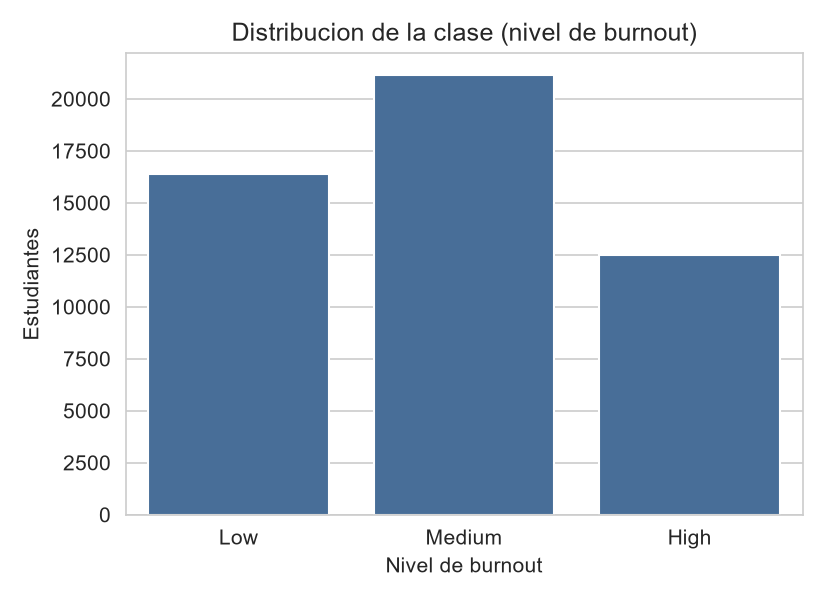
\includegraphics[width=0.5\textwidth]{distribucion_clases.png}
\caption{Distribución de estudiantes por nivel de burnout.}
\label{fig:distribucion}
\end{figure}

\subsection{Análisis exploratorio}
Para entender qué variables se relacionan con el burnout, la Tabla~\ref{tab:medias} compara el promedio de algunas variables entre las tres clases. El patrón más claro es el de las \textbf{horas de IA}: pasan de 4.6 horas semanales en los estudiantes con burnout bajo a \textbf{15.2 horas} en los de burnout alto, más del triple. También sube la dependencia percibida de la IA y, ligeramente, la ansiedad.

\begin{table}[H]
\centering
\caption{Promedio de variables clave según el nivel de burnout.}
\label{tab:medias}
\small
\begin{tabular}{lccc}
\toprule
\textbf{Variable (promedio)} & \textbf{Low} & \textbf{Medium} & \textbf{High} \\
\midrule
Weekly\_GenAI\_Hours       & 4.64  & 7.35  & \textbf{15.21} \\
Traditional\_Study\_Hours  & 11.97 & 11.29 & 10.08 \\
Perceived\_AI\_Dependency  & 2.82  & 3.36  & 4.64 \\
Anxiety\_Level (exámenes)  & 3.93  & 4.17  & 4.89 \\
Skill\_Retention\_Score    & 76.40 & 76.24 & 74.25 \\
\bottomrule
\end{tabular}
\end{table}

La Figura~\ref{fig:boxplot} confirma visualmente esta relación: a mayor nivel de burnout, mayor es la mediana y la dispersión de las horas de IA. Por su parte, la Figura~\ref{fig:correlacion} muestra las correlaciones entre variables numéricas, donde destaca la fuerte relación entre el promedio antes y después del semestre.

\begin{figure}[H]
\centering
\subfigure[Horas de IA por nivel de burnout]{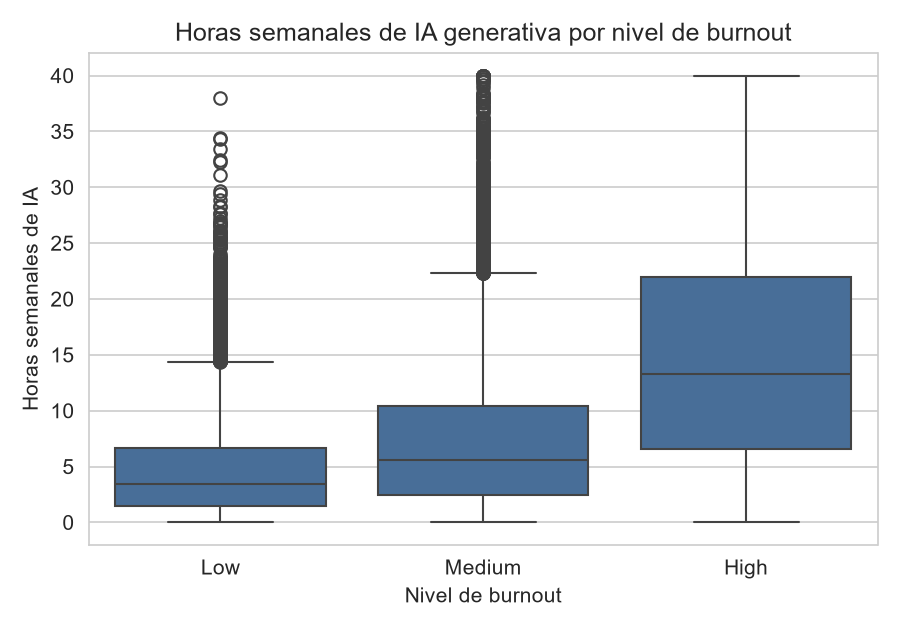
\includegraphics[width=0.47\textwidth]{boxplot_genai.png}\label{fig:boxplot}}
\hfill
\subfigure[Correlación entre variables numéricas]{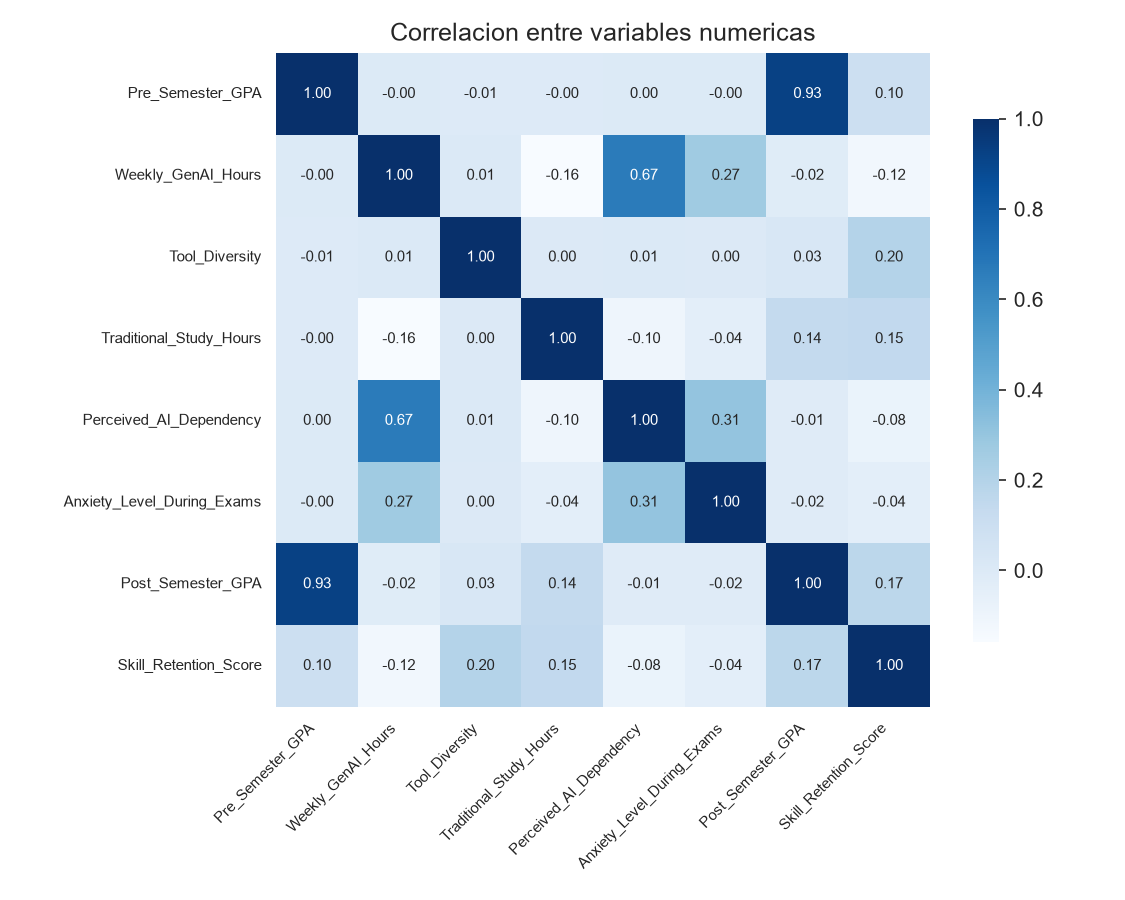
\includegraphics[width=0.47\textwidth]{correlacion.png}\label{fig:correlacion}}
\caption{Análisis exploratorio de las variables numéricas.}
\label{fig:eda}
\end{figure}

\subsection{Transformación de los datos}
Antes de entrenar los modelos se aplicaron tres transformaciones:

\begin{enumerate}[leftmargin=*]
  \item \textbf{Variable derivada.} Se creó \texttt{GPA\_Change} $=$ \texttt{Post\_Semester\_GPA} $-$ \texttt{Pre\_Semester\_GPA}, que resume si el estudiante mejoró o empeoró su promedio durante el semestre.
  \item \textbf{Codificación de categóricas.} Las variables de texto se convirtieron a numéricas mediante \textit{one-hot encoding} (una columna binaria por categoría). Tras este paso, el conjunto pasó a tener \textbf{26 variables predictoras}.
  \item \textbf{División y estandarización.} Los datos se separaron en \textbf{80\,\% para entrenar} (40\,000 ejemplos) y \textbf{20\,\% para probar} (10\,000), de forma \textbf{estratificada} para conservar la proporción de clases. La estandarización se ajustó \textbf{solo con los datos de entrenamiento} y luego se aplicó a los de prueba, para no filtrar información.
\end{enumerate}

\begin{nota}[¿Por qué estandarizar?]
KNN y SVM se basan en distancias, así que una variable con números grandes (como el puntaje de retención, de 0 a 100) pesaría más que otra pequeña (como la diversidad de herramientas, de 1 a 5) sin ninguna razón. La estandarización deja a todas en una escala comparable. El árbol de decisión no lo necesita, porque trabaja con umbrales sobre cada variable por separado.
\end{nota}

% ======================================================================
\section{Aplicación de los Modelos}
\label{sec:modelos}

\subsection{Diseño experimental}
El experimento se implementó en Python con la biblioteca \texttt{scikit-learn}. Los tres modelos se entrenaron sobre los mismos datos de entrenamiento y se evaluaron sobre el mismo conjunto de prueba de 10\,000 ejemplos, para que la comparación fuera justa. Para cada modelo se buscaron sus mejores parámetros con \textbf{validación cruzada de 5 particiones}.

\begin{nota}[SVM sobre una muestra representativa]
Entrenar SVM con kernel RBF sobre las 40\,000 filas de entrenamiento es muy costoso: un solo entrenamiento tarda varios minutos y una búsqueda de parámetros tardaría horas. Por eso, y como se acordó, el SVM se ajustó y entrenó sobre una \textbf{muestra estratificada de 10\,000 ejemplos} del conjunto de entrenamiento. La evaluación se hizo sobre el mismo conjunto de prueba que los otros dos modelos.
\end{nota}

\subsection{Árbol de decisión}
Se probaron distintas profundidades y tamaños mínimos de hoja. La mejor configuración fue \textbf{profundidad máxima 6} y \textbf{mínimo 50 ejemplos por hoja}. La Figura~\ref{fig:importancia} muestra qué variables usa más el árbol para decidir: \texttt{Weekly\_GenAI\_Hours} domina de forma aplastante, con cerca del \textbf{80\,\%} de la importancia total, muy por encima del resto.

\begin{figure}[H]
\centering
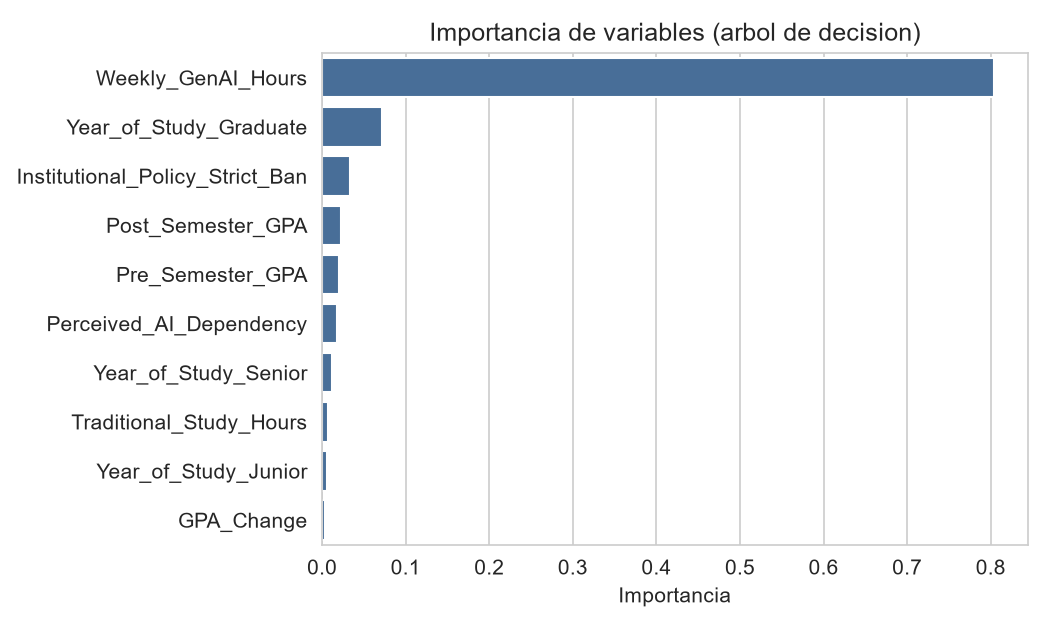
\includegraphics[width=0.72\textwidth]{importancia.png}
\caption{Importancia de las variables en el árbol de decisión.}
\label{fig:importancia}
\end{figure}

\subsection{K-Vecinos más Cercanos (KNN)}
Se evaluaron varios valores de $k$ mediante validación cruzada (Figura~\ref{fig:seleccionk}). La exactitud crece al aumentar $k$ y se estabiliza alrededor de $k=101$, valor que se eligió como el mejor. Que se necesite un $k$ tan grande es una señal de que las clases están muy mezcladas: el modelo necesita observar a muchos vecinos para decidir con cierta estabilidad.

\begin{figure}[H]
\centering
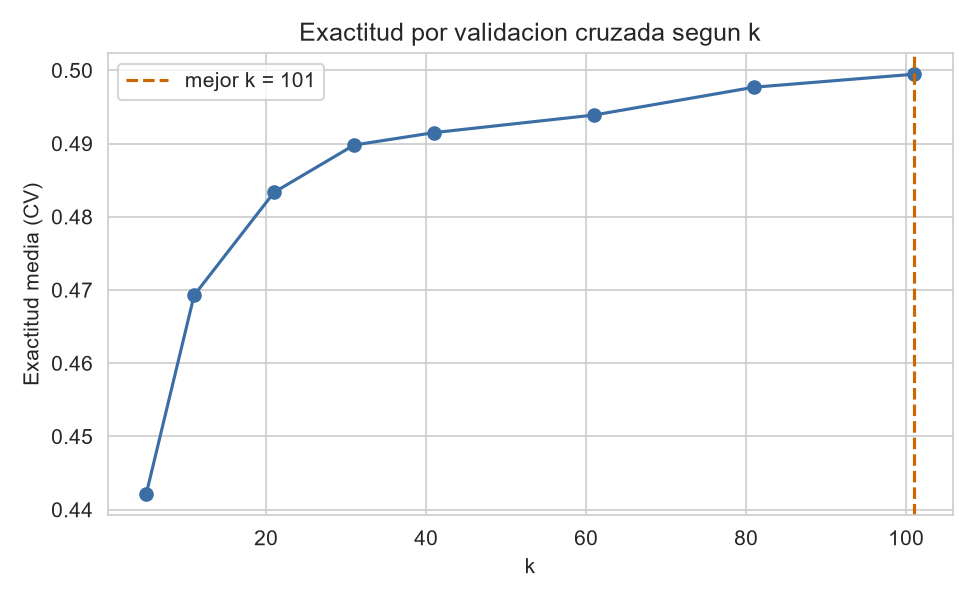
\includegraphics[width=0.68\textwidth]{seleccion_k.png}
\caption{Exactitud media por validación cruzada en función de $k$.}
\label{fig:seleccionk}
\end{figure}

\subsection{Máquinas de Vectores de Soporte (SVM)}
La búsqueda en rejilla sobre la muestra de 10\,000 ejemplos seleccionó un \textbf{kernel RBF} con $C=1$ y $\gamma=$ \texttt{scale}. Esta configuración ofreció el mejor equilibrio entre ajuste y capacidad de generalización.

% ======================================================================
\section{Resultados y Evaluación}
\label{sec:resultados}

\subsection{Comparación de desempeño}
La Tabla~\ref{tab:comparativa} y la Figura~\ref{fig:comparativa} resumen el desempeño de los tres modelos sobre el conjunto de prueba. El \textbf{árbol de decisión} obtuvo el mejor resultado (52.48\,\% de exactitud), seguido muy de cerca por SVM (52.12\,\%) y KNN (50.02\,\%). Las diferencias son pequeñas, lo que indica que ningún algoritmo logra una ventaja clara sobre este problema.

\begin{table}[H]
\centering
\caption{Comparación de los tres modelos sobre el conjunto de prueba (10\,000 instancias).}
\label{tab:comparativa}
\begin{tabular}{lcccc}
\toprule
\textbf{Modelo} & \textbf{Accuracy} & \textbf{Macro F1} & \textbf{T. entren. (s)*} & \textbf{T. predic. (s)*} \\
\midrule
\textbf{Árbol de decisión} & \textbf{0.5248} & \textbf{0.5235} & 0.28 & $<0.01$ \\
SVM (RBF)                  & 0.5212 & 0.5127 & 10.16 & 8.97 \\
KNN ($k=101$)              & 0.5002 & 0.4770 & 0.07 & 6.10 \\
\bottomrule
\end{tabular}
\\[2pt]
{\footnotesize *Los tiempos son aproximados y dependen del equipo; interesa su comparación relativa, no el valor absoluto.}
\end{table}

\begin{figure}[H]
\centering
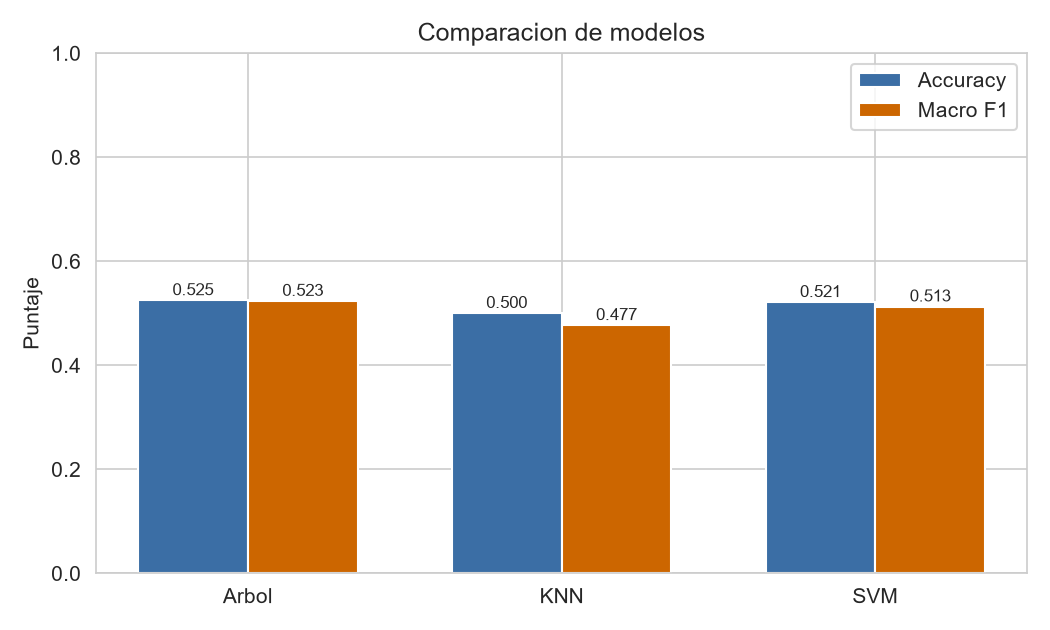
\includegraphics[width=0.68\textwidth]{comparativa.png}
\caption{Comparación de exactitud y \textit{Macro} F1 de los tres modelos.}
\label{fig:comparativa}
\end{figure}

Sobre los tiempos, el árbol es el más práctico: entrena y predice casi al instante. KNN casi no tarda en entrenar (solo guarda los datos), pero es lento al predecir porque debe comparar cada caso con todos los ejemplos. SVM es el más costoso de entrenar, razón por la que se trabajó con una muestra.

\begin{nota}[Sobre el nivel de exactitud]
Un 52\,\% de aciertos puede parecer bajo, pero conviene ponerlo en contexto: al haber \textbf{tres clases}, adivinar al azar acertaría solo alrededor del 33\,\%. Los modelos superan claramente ese punto de partida. Aun así, el techo cercano al 52\,\% ---que se repitió con los tres algoritmos--- indica que el burnout \textbf{solo puede predecirse de forma parcial} con estas variables: buena parte del fenómeno depende de factores personales que el conjunto de datos no captura.
\end{nota}

\subsection{Análisis de las matrices de confusión}
Las Figuras~\ref{fig:cmarbol},~\ref{fig:cmsvm} y~\ref{fig:cmknn} muestran las matrices de confusión de los tres modelos. En todas se repite el mismo patrón: la clase \textit{Medium}, al estar ``en medio'', comparte características con las otras dos y es donde se concentra la mayor confusión. La clase \textit{High} es la que mejor se identifica cuando se predice (alta precisión), aunque muchos de sus casos se escapan hacia \textit{Medium} (baja sensibilidad).

\begin{figure}[H]
\centering
\subfigure[Árbol de decisión]{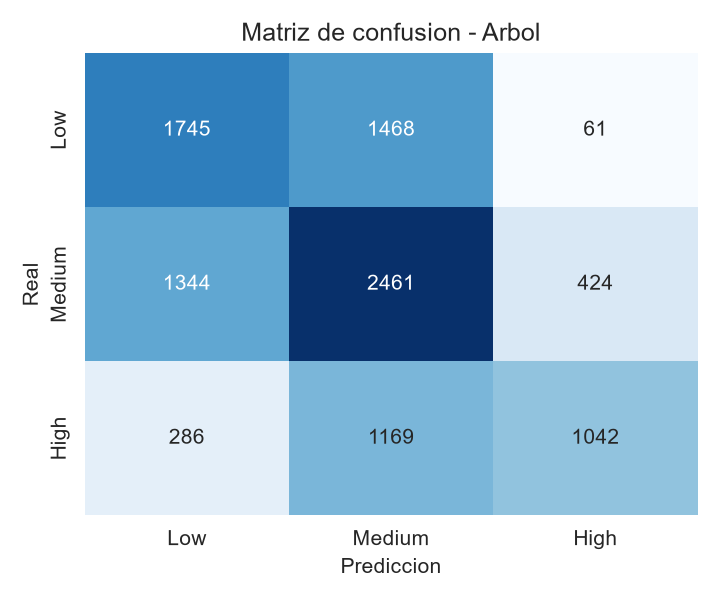
\includegraphics[width=0.32\textwidth]{cm_arbol.png}\label{fig:cmarbol}}
\hfill
\subfigure[SVM (RBF)]{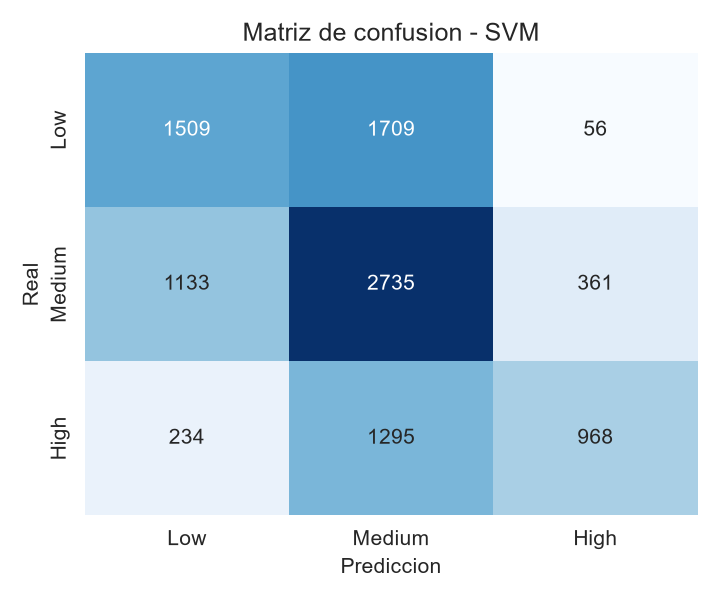
\includegraphics[width=0.32\textwidth]{cm_svm.png}\label{fig:cmsvm}}
\hfill
\subfigure[KNN ($k=101$)]{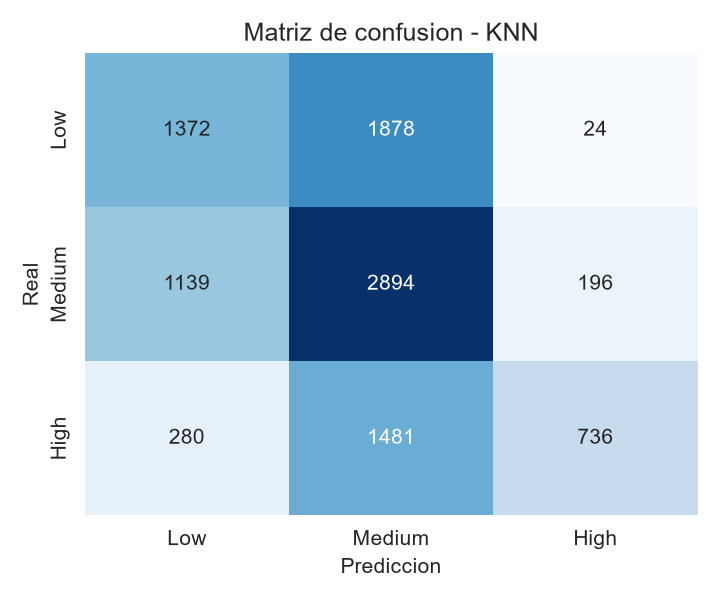
\includegraphics[width=0.32\textwidth]{cm_knn.png}\label{fig:cmknn}}
\caption{Matrices de confusión de los tres modelos sobre el conjunto de prueba.}
\label{fig:matrices}
\end{figure}

\subsection{Métricas por clase}
La Tabla~\ref{tab:porclase} desglosa el F1 por clase para cada modelo. Se aprecia que la clase \textit{Medium} es donde el árbol y el SVM se apoyan más, mientras que KNN, con su $k$ grande, tiende a predecir \textit{Medium} en exceso y por eso baja su desempeño en \textit{High}.

\begin{table}[H]
\centering
\caption{F1-Score por clase para cada modelo.}
\label{tab:porclase}
\begin{tabular}{lccc}
\toprule
\textbf{Modelo} & \textbf{Low} & \textbf{Medium} & \textbf{High} \\
\midrule
Árbol de decisión & 0.5249 & 0.5277 & 0.5179 \\
SVM (RBF)         & 0.4907 & 0.5488 & 0.4987 \\
KNN ($k=101$)     & 0.4524 & 0.5522 & 0.4263 \\
\bottomrule
\end{tabular}
\end{table}

\subsection{Cálculo manual de las métricas}
Al igual que en las actividades anteriores, las métricas se comprobaron \textbf{a mano} a partir de la matriz de confusión, bajo el esquema \textit{una clase contra el resto}. Para cada clase se definen cuatro cantidades ---verdaderos positivos (TP), falsos negativos (FN), falsos positivos (FP) y verdaderos negativos (TN)--- y se aplican las fórmulas vistas en clase:
\begin{equation}
\text{Precisión} = \frac{TP}{TP+FP}, \qquad
\text{Sensibilidad} = \frac{TP}{TP+FN}, \qquad
\text{Especificidad} = \frac{TN}{TN+FP}.
\label{eq:metricas}
\end{equation}

A modo de ejemplo, se desarrolla el cálculo para la clase \textbf{High} del mejor modelo (el árbol de decisión). De su matriz de confusión se obtiene $TP=1042$, $FN=1455$, $FP=485$ y $TN=7018$:

\begin{resultado}
\[
\text{Precisión} = \frac{1042}{1042+485} = 0.6824, \qquad
\text{Sensibilidad} = \frac{1042}{1042+1455} = 0.4173,
\]
\[
\text{Especificidad} = \frac{7018}{7018+485} = 0.9354.
\]
\end{resultado}

Aplicando el mismo procedimiento a las tres clases se obtiene la Tabla~\ref{tab:manualarbol}. La exactitud global se calcula como el total de aciertos (la diagonal de la matriz) entre el total de instancias: $\tfrac{1745+2461+1042}{10\,000}=\tfrac{5248}{10\,000}=0.5248$, que coincide con el valor entregado por la implementación y confirma la consistencia de los resultados.

\begin{table}[H]
\centering
\caption{Cálculo manual de métricas por clase para el árbol de decisión (esquema una contra el resto).}
\label{tab:manualarbol}
\begin{tabular}{lccccccc}
\toprule
\textbf{Clase} & \textbf{TP} & \textbf{FN} & \textbf{FP} & \textbf{TN} & \textbf{Precisión} & \textbf{Sensibilidad} & \textbf{Especificidad} \\
\midrule
Low    & 1745 & 1529 & 1630 & 5096 & 0.5170 & 0.5330 & 0.7577 \\
Medium & 2461 & 1768 & 2637 & 3134 & 0.4827 & 0.5819 & 0.5431 \\
High   & 1042 & 1455 &  485 & 7018 & 0.6824 & 0.4173 & 0.9354 \\
\bottomrule
\end{tabular}
\end{table}

% ======================================================================
\section{Conclusiones}
\label{sec:conclusiones}

Siguiendo la metodología KDD, se logró construir y evaluar un modelo supervisado capaz de predecir el nivel de burnout estudiantil a partir de hábitos de estudio y de uso de IA. Las principales conclusiones son:

\begin{itemize}[leftmargin=*]
  \item El \textbf{árbol de decisión} ofreció el mejor equilibrio entre desempeño, rapidez e interpretabilidad, con una exactitud de \textbf{52.48\,\%} y un \textit{Macro} F1 de \textbf{0.5235}, apenas por encima de SVM y KNN.
  \item El hallazgo más importante del análisis no es tanto el modelo ganador como \textbf{qué variable manda}: el \textbf{número de horas semanales de uso de IA} concentra cerca del 80\,\% de la importancia. Los estudiantes que usan la IA de forma más intensiva tienden a reportar un burnout más alto.
  \item La exactitud, cercana al 52\,\% frente al 33\,\% del azar, muestra que el burnout es \textbf{parcialmente predecible}: estas variables explican una parte del fenómeno, pero no todo. Esto es esperable, ya que el agotamiento también depende de factores personales y de contexto que el conjunto de datos no recoge.
  \item La clase \textit{Medium} es la más difícil de separar por estar ``en medio'' de las otras dos, y es donde se concentra la mayor parte de los errores de los tres modelos.
\end{itemize}

En conjunto, el trabajo cumple el objetivo planteado: más allá del porcentaje de aciertos, el mensaje práctico es que el \textbf{uso intensivo de IA generativa es el factor más asociado al agotamiento} de los estudiantes, un resultado que invita a promover un uso más equilibrado de estas herramientas.

\end{document}
